% !TeX root = ./jvk-blatt1.tex

% l.47 Play-Button
%\usepackage{amssymb};

\newcommand{\jvkpackage}{JavaVorkurs\_EclipseProjekt.zip}
\newcommand{\jvkpackageurl}{https://fius.de/wp-content/uploads/2020/10/JavaVorkurs2020\_EclipseProjekt.zip} % TODO: change URL

\excercise{Programmstart}

\begin{Infobox}[How-To: Install Eclipse]
    \begin{enumerate}[label=\arabic*.]
        \item Schaue das Video des Tutors vorne an und nutze folgenden Link falls du nicht mitgekommen bist:
        \color{blue}\href{https://youtu.be/zxH3G1MTrVs}{\textit{https://youtu.be/zxH3G1MTrVs}}
    \end{enumerate}
\end{Infobox}

\begin{Infobox}[How-To: Wie bekomme ich des Projekt]
    \begin{enumerate}[label=\arabic*.]
        \item Lade zuerst das Maven-Projekt \jvkpackage { }runter, man findet es hier:
        \begin{center}
            \color{blue}\href{\jvkpackageurl}{\textit{\jvkpackageurl}}
        \end{center}

        \item Nachdem das Zip-File heruntergeladen wurde, muss man es in einem geeigneten Ordner entpacken.\\
        \textbf{Windows:} Entpacken funktioniert durch einen Rechtsklick auf die Datei und dann durch klicken auf \fbox{Alle extrahieren...}$\to$\fbox{Extrahieren}.\\
        \textbf{Linux:} Am schnellsten entpackt man ein Zip-File über das Terminal mit dem Befehl:
        \newline\hspace*{\fill}\texttt{\textgreater\ unzip \jvkpackage}\hspace*{\fill}\newline
        \textbf{Apple:} Nachdem man das Zip-File im Finder offen hat, entpackt man es durch einen einfachen Doppelklick.
    \end{enumerate}
\end{Infobox}


\begin{Infobox}[How-To: Projekt Import in Eclipse]
    \begin{enumerate}[label=\arabic*.]
        \item Um ein Projekt zu importieren, klicke zuerst auf \fbox{File} $\to$ \fbox{Import...}.
        \item Wähle in der Auswahl \fbox{Maven} $\to$ \fbox{Existing Maven Projects} oder nutze das Suchfeld oben um \fbox{Existing Maven Projects} zu finden. Klicke dann auf \fbox{Next \textgreater}.
        \item Drücke oben rechts auf \fbox{Browse...} und suche das Verzeichnis, in welchem die Datei \jvkpackage { }entpackt wurde.
        \item Stelle sicher, dass der Projektname im \textit{Projects} Bereich des Fensters auftaucht.
        \item Zu guter Letzt noch auf \fbox{Finish} drücken.
        \item Nachdem sich das Fenster geschlossen hat, siehst du das Projekt im \textit{Package Explorer} links an der Seite.
        \item Damit euer Projekt richtig funktioniert, solltet ihr im \textit{Package Explorer} das Projekt mit einem Rechtsklick auswählen und dann im Kontextmenü \fbox{Maven} $\to$ \fbox{Update Project...} $\to$ \fbox{OK} ausführen.
    \end{enumerate}
\end{Infobox}


\newpage

Öffne nun die Entwicklungsumgebung Eclipse und importiere das heruntergeladene Maven-Projekt \jvkpackage { } wie oben in den beiden HowTo's beschrieben.

\begin{enumerate}
    \item
    \begin{itemize}
        \item Öffne die \texttt{Main}-Datei in dem Dateiexplorer auf der linken Seite. Navigiere dazu in den \texttt{src/main/java} Ordner und wähle dann das Paket \texttt{de.unistuttgart.informatik.fius.jvk} aus.
        \item Starte als nächstes das Projekt, um zu schauen ob alles klappt. Drücke dazu den grünen Play Button $\vartriangleright$ oben links.
        \item Wenn Du bei der Installation alles Richtig gemacht hast, sollten nun keine Fehler (roter Text) auftreten. Da wir noch nichts programmiert haben, sollte aber auch sonst nichts passieren.
        \begin{center}
            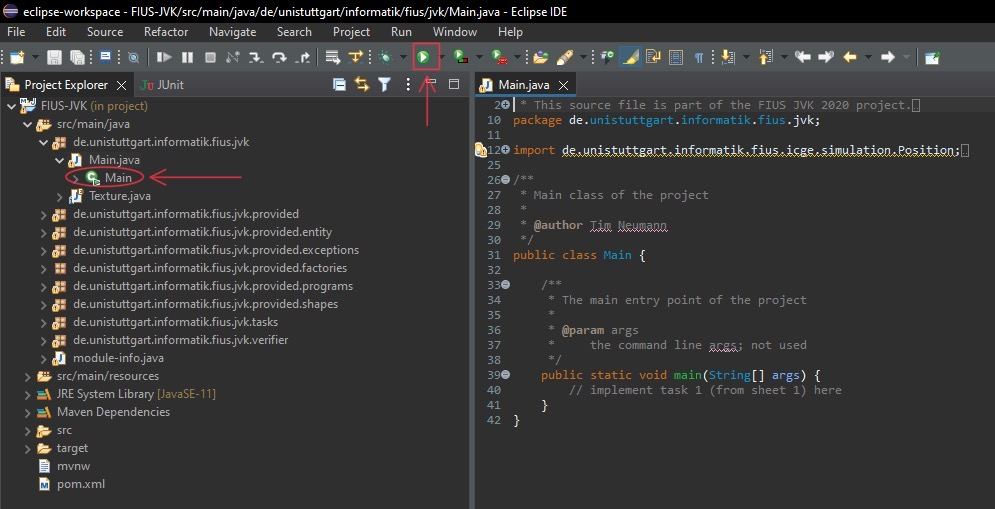
\includegraphics[width=\linewidth]{./figures/ide.jpg} % Todo Pfeile einfügen
        \end{center}
    \end{itemize}

    \item Finde in der \lstinline{Main} Klasse die Zeile mit \lstinline{// implement task 1 (from sheet 1) here} und füge an seiner Stelle den fehlenden Code aus dem Bild ein.
    Aktuell musst du den Code noch nicht verstehen, es geht darum den Code Editor in Eclipse kennenzulernen.
    Achte also darauf was passiert während du die fehlenden Zeilen eingibst.

    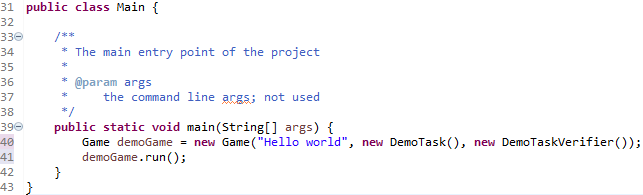
\includegraphics[width=\linewidth]{./figures/code.1.png}

    Wenn das Programm jetzt ausgeführt wird geht ein Fenster mit der Simulator Ansicht auf.
    Suche nun die (rote) Stop Taste in Eclipse um das Programm abzubrechen.
    Die Taste befindet sich in Eclipse unten in der Titelleiste der Console.
    \item Versuche nun den Code so zu verändern, dass dein Name im Fenstertitel steht.
\end{enumerate}


\begin{Infobox}[HowTo: Auskommentieren]
    Manchmal möchte man, dass bestimmter Code nicht ausgeführt wird. Vielleicht möchten man ihn erst später ausführen, ihn einfach nicht verlieren oder etwas Neues ausprobieren.
    In solchen Fällen Kommentieren wir die Code-Zeilen einfach aus.
    Dies geht, indem wir der Code-Zeile zwei Schrägstriche (\emph{eng.} slashes)(\lstinline{//}) voranstellen.
    Als Beispiel betrachten wir mal den folgenden Code:\\

    \hfill
    \begin{minipage}{.96\textwidth}
        \begin{lstlisting}
public void run(Simulation sim) {
    PlayfieldModifier pm =
            new PlayfieldModifier(sim.getPlayfield());
    pm.placeEntityAt(new Coin(), new Position(0, 0));
}
        \end{lstlisting}
    \end{minipage}

    Wenn wir nun die letzte Zeile auskommentieren wollen, dann stellt sich der Code wie folgt dar.\\

    \hfill
    \begin{minipage}{.96\textwidth}
        \begin{lstlisting}
public void run(Simulation sim) {
    PlayfieldModifier pm =
            new PlayfieldModifier(sim.getPlayfield());
    //pm.placeEntityAt(new Coin(), new Position(0, 0));
}
        \end{lstlisting}
    \end{minipage}

    Alles ab den zwei Schrägstrichen bis zum Zeilen Ende wird nun vom Computer ignoriert, was durch eine andere Färbung in Eclipse deutlich wird.
\end{Infobox}


\begin{Infobox}[Fehler]
    Einige Aufgaben in Blatt 1 (und auch den anderen Blättern) verlangen von euch, den Code absichtlich kaputt zu machen.
    Ziel davon ist es das ihr die verschiedenen Fehler bereits kennenlernt.
    Achtet also bei solchen Aufgaben darauf, welche Änderung zu welchem Fehler geführt hat.
    Falls ihr nun später einen Fehler beim Programmieren macht, kann euch dieses Wissen helfen den Code zu reparieren.

    Ihr braucht auch keine Angst haben, dass ihr etwas nachhaltig kaputt machen könntet.
    Eclipse hat eine \q{Undo}-Funktion welche Änderungen rückgängig macht. Diese findet ihr im Menü oben unter \fbox{edit} (deutsch \fbox{Bearbeiten}) oder über \fbox{Strg + z} aufrufen könnt.
    Falls ihr trotzdem Hilfe braucht, könnt (\emph{und sollt!}) ihr euch gerne bei den Tutoren melden.
\end{Infobox}


\begin{enumerate} \setcounter{enumi}{3}
\item Finde heraus was passiert, wenn man die erste oder die zweite Zeile in der Main-Funktion auskommentiert.

Hinweis: Nicht alle Varianten funktionieren zwangsläufig, Überlege warum dies der Fall sein könnte.
\item Vielleicht sind dir beim Ausprobieren in a) schon einige Dinge aufgefallen die der Eclipse Editor anders macht als Textverarbeitungsprogramme, wie zum Beispiel Word.
Wenn du \lstinline{demoGame.} eingibst erscheint ein \textit{Overlay} mit möglichen \textit{Autocompletions}.
Wenn du dann mit der Maus über andere Stellen im Code gehst, verschwindet das Overlay wieder.
Öffne das Overlay manuell, indem du den Cursor direkt nach \lstinline{demoGame.} platzierst und \fbox{Strg + Space} (Space ist die Leertaste) drückst.
\item
Wenn du die Maus über \lstinline{Game} bewegst, siehst du ein Overlay mit der Dokumentation.
Das funktioniert auch an anderen Stellen im Code.
Was steht im Overlay von \lstinline{DemoTask()}? Sollte sich das Overlay nicht öffnen, dann kannst du \fbox{F2} drücken
\item
Wenn du \fbox{Strg + Shift + f} (Shift ist die Taste mit der man Großbuchstaben schreibt) drückst, formatiert Eclipse den Code für dich.
Füge an verschiedenen Stellen neue Zeilen und Leerzeichen ein und beobachte was passiert, wenn du \fbox{Strg + Shift + f} drückst
\end{enumerate}


\begin{Infobox}[Optionale Aufgaben]
    Aufgaben die mit \optional markiert, sind müssen nicht bearbeitet werden.
    Sie setzen schon Vorkenntnisse in Java oder Programmieren vorraus und sind deshalb auch oft deutlich schwerer als die normalen Aufgaben.
    Wenn du also an einer optionalen Aufgabe festhängst, dann solltest du mit der nächsten normalen Aufgabe weitermachen.
    Später, wenn du genug Zeit oder Wissen hast um die optionale Aufgabe zu lösen, kannst du nochmal zu ihr zurückkehren.
\end{Infobox}


\begin{enumerate} \setcounter{enumi}{5}
\item \optional Finde eine Möglichkeit, den Fenstertitel nach der \lstinline{demoGame.run();} Zeile zu ändern.
Dafür benötigst du den folgenden Code, den du aber noch auf deinen Namen anpassen musst: \lstinline{demoGame.getGameWindow().setWindowTitle("");}
\item \optional Benenne \lstinline{demoGame} in \lstinline{myDemoGame} um.
Wenn du nur die Stelle \lstinline{Game demoGame} anpasst, wirst du eine Fehlermeldung bekommen.
Mache deine Änderung nochmal rückgängig und platziere den Cursor in dem Wort \lstinline{demoGame}.
Mit der Tastenkombination \fbox{Shift + Alt + r} kommst du in den \q{Refactor}-Modus, in dem du alle Vorkommen des Namens gleichzeitig umbenennen kannst.
Das gleiche geht auch über Rechtsklick > \fbox{Refactor} > \fbox{Rename}.

Mit \fbox{Strg + Shift + l} kannst du eine Liste alle Tastenkombinationen ansehen.
\item \optional Versuche, drei Fenster gleichzeitig zu starten.
\end{enumerate}
